% !TeX root = ../main.tex
% Add the above to each chapter to make compiling the PDF easier in some editors.

\chapter{Approximative Offline Scheduling}
Heretofore, we have derived two optimal offline algorithms for our scheduling problem. Unfortunately, the algorithm's runtime complexities are exponential in the input size of the number of servers $m$. Needless to say, we want to reduce this exponential runtime. For this, we must slightly loosen our aspirations, that is we move to approximative methods. Further, as we will see in the next section, we need to assume that our convex operating costs function $f$ is monotonically increasing; however, this restriction is of no great significance since in practice most operating costs functions fulfill this requirement.\unsure{Any reference?} 

In this chapter, we will first modify our algorithm derived in Section~\ref{sec:opt_offline_pseudo_lin} to obtain a 3-optimal offline algorithm with linear runtime complexity. As a next step, we will generalize our first approach to allow for arbitrary $1+\beps$-approximations with TODO complexity.

\section{A 3-Optimal Algorithm}
Recall our algorithm and its corresponding graph $G$ derived in Section~\ref{sec:opt_offline_pseudo_lin}. The algorithm's runtime complexity of $\Theta(Tm)$ is determined by the number of nodes and edges of $G$. Since we desire to reduce our runtime complexity, we need to reduce the number of nodes and edges in $G$. In particular, we must get rid of the factor $m$. This factor is a consequence of the ``height'' of our graph, that is the number of nodes in each layer. Therefore, we have to ``thin out'' $G$ by reducing its number of nodes in each layer.

As we saw in Equation~\eqref{eq:inp_size}, the size of our input $\inp$ is given by $\mathcal{O}\bigl(T\log_2(m)+\log_2(\beta)\bigr)$. Consequently, in order to obtain a linear runtime complexity, we want to reduce the graph's height from $m+1$ to a logarithmic height of $\mathcal{O}\bigl(\log(m)\bigr)$. Given this observation, it seems natural for a computer scientist to choose a logarithmic scale for the number of servers in each layer; that is, instead of adding a node for each possible number of active servers (i.e.\ $0,1,\ldots,m$), we only add nodes for logarithmic choices (i.e.\ $0,2^0,2^1,\ldots,2^{\lfloor\log_2(m)\rfloor},m$). More formally, given a problem instance $\inp$, we set
\begin{align*}
	b&\coloneqq\lfloor\log_2(m)\rfloor\\
	B&\coloneqq\{0,2^0,2^1,\ldots,2^b,m\}
\end{align*}
where $B$ will subsequently represent the set of possible scheduling choices at each time slot. Using this set of possible choices, we can then consider the following adaption of our former graph:
\begin{align*}
	V&\coloneqq\bigl\{v_{x,t\downarrow}\mid x\in B,t\in[T]\bigr\}\dotcup\bigl\{v_{x,t\uparrow}\mid x\in B, t\in[T-1]\bigr\}\dotcup\{v_{0,0}\}\\
	E_s&\coloneqq\bigl\{(v_{0,0},v_{x,1\downarrow})\mid x\in B\bigr\}\\
	E_\downarrow&\coloneqq\bigl\{(v_{2^i,t\downarrow},v_{2^{i-1},t\downarrow})\mid i\in[b],t\in[T]\bigr\}\dotcup\bigl\{(v_{2^0,t\downarrow},v_{0,t\downarrow})\mid t\in[T]\bigr\}\dotcup\\
	&\phantom{{}\coloneqq{}}\bigl\{(v_{m,t\downarrow},v_{2^b,t\downarrow})\mid t\in[T]\bigr\}\\
	E_\uparrow&\coloneqq\bigl\{(v_{2^{i-1},t\uparrow},v_{2^i,t\uparrow})\mid i\in[b],t\in[T-1]\bigr\}\dotcup\bigl\{(v_{0,t\uparrow},v_{2^0,t\uparrow})\mid t\in[T-1]\bigr\}\dotcup\\
	&\phantom{{}\coloneqq{}}\bigl\{(v_{2^b,t\uparrow},v_{m,t\uparrow})\mid t\in[T-1]\bigr\}\\
	E_{\downarrow\uparrow}&\coloneqq\bigl\{(v_{x,t\downarrow},v_{x,t\uparrow})\mid x\in B,t\in[T-1]\bigr\}\\
	E_{\uparrow\downarrow}&\coloneqq\bigl\{(v_{x,t\uparrow},v_{x,t+1\downarrow})\mid x\in B,t\in[T-1]\bigr\}\\
	E&\coloneqq E_s\dotcup E_\downarrow\dotcup E_\uparrow\dotcup E_{\downarrow\uparrow}\dotcup E_{\uparrow\downarrow}\\
	c_G(e)&\coloneqq
	\begin{cases}
		\costs(0,x,\lambda_1), & \text{if $e=(v_{0,0},v_{x,1\downarrow})\in E_s$}\\
		\opcosts(x,\lambda_{t+1}), & \text{if $e=(v_{x,t\uparrow},v_{x,t+1\downarrow})\in E_{\uparrow\downarrow}$}\\
		(x'-x)\beta, & \text{if $e=(v_{x,t\uparrow},v_{x',t\uparrow})\in E_\uparrow$}\\
		0, & \text{if $e\in(E_\downarrow\dotcup E_{\downarrow\uparrow})$}
	\end{cases}\\
	G&\coloneqq(V,E,c_G)
\end{align*}
A more appealing, graphical representation can be found in the following figure.
\begin{figure}[H]
\centering
\resizebox{\textwidth}{!}{
\begin{tikzpicture}[->,>=stealth',auto,node distance=2.2cm,thick,node/.style={minimum size=1.5cm,circle,draw}]
  \node[node] (1) {0,0};
  \node[node] (4) [below right=4cm of 1] {0,1$\downarrow$};
  \node[node] (3) [above =0.5cm of 4] {$2^0$,1$\downarrow$};
  \node[node] (2) [above right=4cm of 1] {m,1$\downarrow$};
  \node[node] (5) [below =0.5cm of 2] {$2^b$,1$\downarrow$};
  \node[node] (7) [right =of 3] {$2^0$,1$\uparrow$};
  \node[node] (6) [right =of 2] {m,1$\uparrow$};
  \node[node] (8) [right =of 4] {0,1$\uparrow$};
  \node[node] (9) [right =of 5] {$2^b$,1$\uparrow$};
  \node[node] (11) [right =of 7] {$2^0$,2$\downarrow$};
  \node[node] (10) [right =of 6] {m,2$\downarrow$};
  \node[node] (12) [right =of 8] {0,2$\downarrow$};
  \node[node] (13) [right =of 9] {$2^b$,2$\downarrow$};
  \node[node] (15) [right =of 11] {$2^0$,2$\uparrow$};
  \node[node] (14) [right =of 10] {m,2$\uparrow$};
  \node[node] (16) [right =of 12] {0,2$\uparrow$};
  \node[node] (17) [right =of 13] {$2^b$,2$\uparrow$};
  \node[node] (19) [right =5cm of 15] {$2^0$,T$\downarrow$};
  \node[node] (18) [right =5cm of 14] {m,T$\downarrow$};
  \node[node] (20) [right =5cm of 16] {0,T$\downarrow$};
  \node[node] (21) [right =5cm of 17] {$2^b$,T$\downarrow$};

  \node (22) at ($(2)!.5!(4)$) {};
  \node (23) at ($(2)!.487!(4)$) {\vdots};
  \node (24) at ($(6)!.487!(8)$) {\vdots};
  \node (25) at ($(10)!.487!(12)$) {\vdots};
  \node (26) at ($(14)!.487!(16)$) {\vdots};
  \node at ($(18)!.487!(20)$) {\vdots};
  \node at ($(23)!.487!(24)$) {\vdots};
  \node at ($(24)!.487!(25)$) {\vdots};
  \node at ($(25)!.487!(26)$) {\vdots};

  \node (27) at ($(14)!.5!(18)$) {\ldots};
  \node at ($(15)!.5!(19)$) {\ldots};
  \node (28) at ($(16)!.5!(20)$) {\ldots};
  \node at ($(17)!.5!(21)$) {\ldots};
  \node at ($(27)!.5!(28)$) {\ldots};

  \path[every node/.style={font=\sffamily\small}]
    (1) edge[red] node[black,above left] {$\costs(0,m,\lambda_1)$} (2)
	edge node[label={[xshift=0.8cm, yshift=-0.9cm]$\costs(0,2^b,\lambda_1)$}] {} (5)
	edge node[above right=-0.13cm] {$\costs(0,2^0,\lambda_1)$} (3)
	edge node[below left] {$\costs(0,0,\lambda_1)$} (4)
    (1) edge ($(1)!.82!(22)$)

    (2) edge node[above] {$0$} (6)
    (3) edge node[above] {$0$} (7)
    (4) edge[red] node[black,above] {$0$} (8)
    (5) edge node[above] {$0$} (9)

    (2) edge[red] node[black,right] {$0$} (5)
    (3) edge[red] node[black,right] {$0$} (4)

    (9) edge[red] node[black,right] {$(m-2^b)\beta$} (6)
    (8) edge[red] node[black,right] {$\beta$} (7)

    (6) edge[red] node[black,above] {$\opcosts(m,\lambda_2)$} (10)
    (7) edge node[above] {$\opcosts(2^0,\lambda_2)$} (11)
    (8) edge node[above] {$\opcosts(0,\lambda_2)$} (12)
    (9) edge node[above] {$\opcosts(2^b,\lambda_2)$} (13)

    (10) edge node[above] {$0$} (14)
    (11) edge node[above] {$0$} (15)
    (12) edge[red] node[black,above] {$0$} (16)
    (13) edge node[above] {$0$} (17)

    (10) edge[red] node[black,right] {$0$} (13)
    (11) edge[red] node[black,right] {$0$} (12)

    (17) edge[red] node[black,right] {$(m-2^b)\beta$} (14)
    (16) edge[red] node[black,right] {$\beta$} (15)

    (5) edge[red] node[black,right] {$0$} ($(5)!.35!(3)$)
    ($(5)!.65!(3)$) edge[red] node[black,right] {$0$} (3)

    ($(7)!.65!(9)$) edge[red] node[black,right] {$2^{b-1}\beta$} (9)
    (7) edge[red] node[black,right] {$2^0\beta$} ($(7)!.35!(9)$)
 
    (13) edge[red] node[black,right] {$0$} ($(13)!.35!(11)$)
    ($(13)!.65!(11)$) edge[red] node[black,right] {$0$} (11)

    ($(15)!.65!(17)$) edge[red] node[black,right] {$2^{b-1}\beta$} (17)
    (15) edge[red] node[black,right] {$2^0\beta$} ($(15)!.35!(17)$)


    (14) edge[red] node[label={[black,xshift=0cm, yshift=-0.26cm]$\opcosts(m,\lambda_3)$}] {} ($(14)!.4!(18)$)
    (15) edge node[label={[xshift=0cm, yshift=-0.26cm]$\opcosts(2^0,\lambda_3)$}] {} ($(15)!.4!(19)$)
    (16) edge node[label={[xshift=0cm, yshift=-0.26cm]$\opcosts(0,\lambda_3)$}] {} ($(16)!.4!(20)$)
    (17) edge node[label={[xshift=0cm, yshift=-0.26cm]$\opcosts(2^b,\lambda_3)$}] {} ($(17)!.4!(21)$)

    ($(14)!.6!(18)$) edge[red] node[black,above] {$\opcosts(m,\lambda_T)$} (18)
    ($(15)!.6!(19)$) edge node[above] {$\opcosts(2^0,\lambda_T)$} (19)
    ($(16)!.6!(20)$) edge node[above] {$\opcosts(0,\lambda_T)$} (20)
    ($(17)!.6!(21)$) edge node[above] {$\opcosts(2^b,\lambda_T)$} (21)

    (18) edge[red] node[black,right] {$0$} (21)
    (19) edge[red] node[black,right] {$0$} (20)
    (21) edge[red] node[black,right] {$0$} ($(21)!.35!(19)$)
    ($(21)!.65!(19)$) edge[red] node[black,right] {$0$} (19);
\end{tikzpicture}
}
\caption{Graph for a linear, 3-optimal offline algorithm; the path of the topological sorting is highlighted in red. Note that $(2^i-2^{i-1})\beta =2^{i-1}\beta$.}
\label{fig:graph_pseudo_lin}
\end{figure}
The nodes' and edges' semantical meaning and the graph's working principle stays similar to that given in Section~\ref{sec:opt_offline_pseudo_lin}. Again, by following the colored path of the topological sorting, we can work our way through the graph to calculate the shortest paths, ultimately reaching the destination $v_{0,T\downarrow}$. Since some possible scheduling choices, however, are not representable in this new graph, we may just obtain approximative costs for our nodes. In order to establish the graph's approxmation guarantee, we first have to conduct some observations.

First, we shall take a look on the incurring operating costs of an approxmative schedule $\mx'$ representable in $G$. Since we are forced to schedule a number of servers contained in $B$, we may not be able to choose an optimal scheduling choice that minimizes the schedule's operating costs. Instead, we may choose the nearest scheduling choice which is contained in $B$. For instance, if the optimal scheduling choice at some timeslot $t$ would be to choose $x_t=3$ servers (which is not a power of two), we may instead have to choose $x_t'=4\in B$ servers in our approximative schedule. One might suspect that this strategy would incur at most twice as much operating costs as the optimal schedule. This, however, is sadly not the case as one can see in the following example.
\begin{exmpl}
Let $\inp=\bigl(m=4,T=5,\Lambda=(3,3,3,3,3),\beta=0,f\bigr)$ be the input for a problem instance where $f(\lambda)=(\lambda-1)^2$. Since we need at least 3 active servers at any timeslot, any approximative schedule $\mx'=(x_1',\ldots,x_5')$ forces us to constantly use $x_t'=4$ active machines. An optimal schedule $\mx=(x_1,\ldots,x_5)$, on the other hand, is able to minimize its costs by constantly scheduling $x_t=3$ servers. Let us compare the costs between $\mx'$ and $\mx$. The schedules' costs are given by
\begin{align*}
	\costs(\mx)&\stackrel{\eqref{eq:mx_schedule_total_costs}}{=}\sum\limits_{t=1}^{5}\bigl(\overbrace{x_t(\lambda_t/x_t-1)^2}^{3(3/3-1)^2}+\overbrace{\beta}^{0}\max\{0,x_t-x_{t-1}\}\bigr)=5\cdot3\Bigl(\frac{3}{3}-1\Bigr)^2=0\\
	\costs(\mx')&\stackrel{\eqref{eq:mx_schedule_total_costs}}{=}\sum\limits_{t=1}^{5}\bigl(\overbrace{x_t'(\lambda_t/x_t'-1)^2}^{4(3/4-1)^2}+\overbrace{\beta}^{0}\max\{0,x_t'-x_{t-1}'\}\bigr)=5\cdot4\Bigl(\frac{3}{4}-1\Bigr)^2=\frac{20}{16} 
\end{align*}
Albeit our approximative schedule uses only one server in addition, the schedule's cost is already inestimably higher than that of an optimal schedule $\mx$, preventing any sensible approximation estimation. Naturally, we may ask ourselves how this explosion of costs is even possible. Evidently, the switching costs are not the root of this explosion since $\beta=0$. Thus, we shall take a closer look on the used operating costs function. The optimal schedule $\mx$ evenly distributes every load $\lambda_t=3$ to $x_t=3$ servers. Hence, every active server has to process a load of $\frac{\lambda_t}{x_t}=1$ at every time step, incurring costs of $f(1)=0$. On the other hand, the approximative schedule $\mx'$ is able to distribute every load to 4 active machines. Thus, every machine incurs costs of $f(\frac{3}{4})=\frac{1}{16}$. This observation seems rather surprsing: Although every server has to process a smaller load using $\mx'$, the incurred operating costs of each server turn out to be higher. Intuitevly, however, we would expect that a less stressed machine would incur less costs. This surprising behavior is due to the fact that our operating costs function $f$ is not monotonically increasing, as one can see in the following figure.
\begin{figure}[H]
\centering
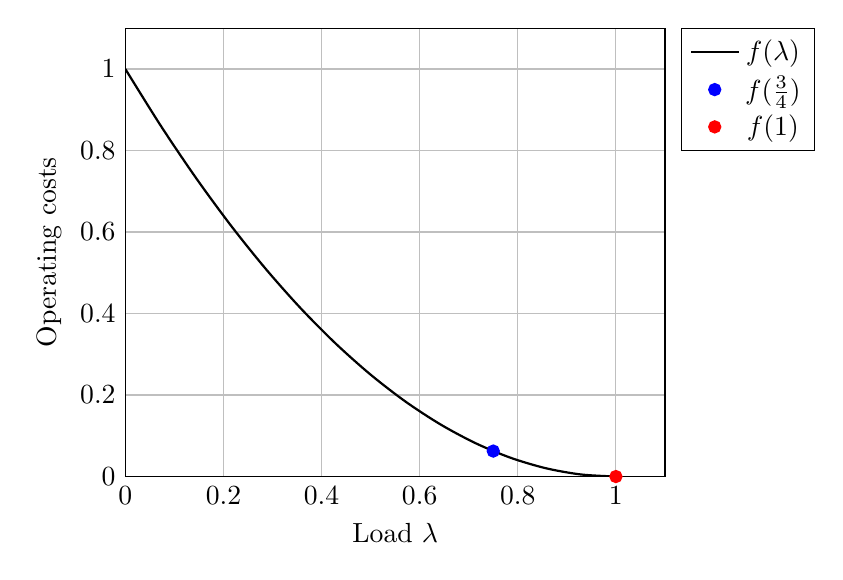
\begin{tikzpicture}
	\begin{axis}[grid=both,tick style={draw=none},every axis plot/.style={
	    domain=0:1,samples=15,smooth,thick}, 
	    xlabel=Load $\lambda$,
	    ylabel=Operating costs,
	    enlargelimits=upper,
	    legend pos=outer north east
	    ]
	\addplot[mark=none,color=black]{(x-1)^2}; 
	\addlegendentry{$f(\lambda)$};
	\addplot [only marks, mark=*,color=blue] coordinates {(0.75,0.0625)};
	\addlegendentry{$f(\frac{3}{4})$};
	\addplot [only marks, mark=*,color=red] coordinates {(1,0)};
	\addlegendentry{$f(1)$};
	\end{axis}
\end{tikzpicture}
\caption{Example of a non-monotonically increasing cost function $f(\lambda)=(\lambda-1)^2$, where smaller loads incur higher costs.}
\label{fig:non_mono_incr_f}
\end{figure}
\end{exmpl}
The above example shows us that our graph may not able to deliver a sensible approximation when dealing with general convex cost functions. However, this inconvenience can solved by using monotonically increasing convex cost functions $f$. To see this, assume that at some timeslot $t$ the scheduling choice $x_t$ minimizes the operating costs to process the load $\lambda_t$. Then let $x_t'\in B$ the next scheduling choice representable in $G$. Since $B$ contains all powers of 2, we have $x_t\le x_t'\le 2x_t$.
\begin{equation*}
	f(\lambda_t/x_t)\stackrel{\text{f monotone increasing}}{\le}f(\lambda_t/x_t')\
\end{equation*}

We thus subsequently restrict ourselves to monotonically increasing convex cost functions.

One might suspect that we are able to obtain 2-optimal costs using our new graph. Sadly, this is not the case, as the next example will show us.
\begin{exmpl}
Let $\inp=\bigl(m=8,T=5,\Lambda=(5,3,5,3,5),\beta=1,f\bigr)$ be the input for a problem instance where $f(\lambda)=1$. Our possible scheduling choices are then given by $B=\{0,1,2,4,8\}$. Since we need at least 5 active servers at timeslots $t\in\{1,3,5\}$, our approximation forces us to use 8 active servers at these slots. If we try to obtain a 2-optimal schedule, we are further forced to use 4 active servers at timeslots $t\in\{2,4\}$ since 
\end{exmpl}

TODO: examples for idea + monotonically increasing f.

Our next task shall be the verification of our new construction. Naturally, since we are not able to represent every schedule in our graph $G$ anymore, we will have to restrict ourselves to the set of schedules respresentable in $G$. For this, we first make a convenient definition.
\begin{defn}[Restricted schedules]
Given an input $\inp$ and a set $A\subseteq\fromto{0}{m}$, we say that a schedule $\mx=(x_1,\ldots,x_T)$ is \textit{$A$-restricted} if $\mx$ only uses scheduling coices contained in $A$, that is $\mx$ satisfies $\forall t\in[T](x_t\in A)$.
\end{defn}
For the next lemma, we need to recall our notion of ``maximum'' nodes $x_t$ in reasonable paths $P$ described in Definition~\ref{defn:max_path_node} as well as that $B=\{0,2^0,2^1,\ldots,2^b,m\}$. Like in Section~\ref{sec:opt_offline_pseudo_lin}, we want to first establish a bijection between $B$-restricted schedules and reasonable paths.
\begin{lem}\label{lem:sched_reasn_path_approx_3}
Let $\bm{\mx}$ be the set of all $B$-restricted schedules for $\inp$, and let $\bm{\mathcal{P}}$ be the set of all reasonable paths. The map
\begin{equation*}
	\Phi:\bm{\mathcal{P}}\rightarrow\bm{\mx},\quad P\mapsto (x_1,\ldots,x_T)
\end{equation*}
is a bijection satisfying $\costs(P)=\costs\bigl(\Phi(P)\bigr)$.
\end{lem}
\begin{proof}
The proof is analogous to the proof of Lemma~\ref{lem:sched_reasn_path_pseudo_lin} considering that we conduct logarithmic instead of incremental switching steps.\unsure{Is this okay?}
\end{proof}
Since we did not change the graph's principle structure, the proof of Lemma~\ref{lem:sched_reasn_path_approx_3} required no new efforts. The next lemma, however, demands more ingenuity. We want to prove that we are able to transform any arbitrary schedule to a $B$-restricted one with a cost factor of at most 3. This will then allow us to verify that our graph is indeed able to produce 3-optimale schedules.
\begin{lem}\label{lem:transform_schedule_approx_3}
Let $\mx$ be a schedule for $\inp$. There exists a 3-approximative $B$-restricted schedule $\mx'$ satisfying \makebox{$\costs(\mx')\le3\costs(\mx)$}.
\end{lem}
\begin{proof}
For $t\in[T]$, we inductively define our new schedule $\mx'\coloneqq(x_1',\ldots,x_T')$ by
\begin{align}
		x'_0&\coloneqq 0\nonumber\\
		x'_t&\coloneqq 
		\begin{cases}
			\min\Bigl\{m,\max\bigl\{x_{t-1}',2^{\lceil \log_2(x_t)\rceil}\bigr\}\Bigr\}, & \text{if }0\le x_{t-1}<x_t\\
			x'_{t-1}, & \text{if $0<x_t\le x_{t-1}$ and }x'_{t-1}\le 3x_t\\
			2^{\lceil \log_2(x_t)\rceil}, & \text{if $0<x_t\le x_{t-1}$ and }x'_{t-1}>3x_t\\
			0, & \text{if }x_t=0
		\end{cases} \label{eq:xprime_approx_3}
\end{align}
We have to define a token payment function. Since we want to be to spare up the unused potential. Thus, we define our token payment function as
\begin{equation}
	\Delta(t)=\begin{cases}
		3\beta(x_t-x_{t-1})-\beta(x_t'-x_{t-1}'), & \text{if }x_{t-1}<x_t\\
		0, & \text{if }x_t\le x_{t-1}\label{eq:delta_approx_3}
	\end{cases}
\end{equation}
Using this definition, we can calculate our amortized switching costs for $\mx'$: 
\begin{equation}
	\aswcosts(x_{t-1}',x_t')=\swcosts(x_{t-1}',x_t')+\Delta(t)\stackrel{\eqref{eq:mx_schedule_sw_costs}}{=}\beta\max\{0,x_t'-x_{t-1}'\}+\Delta(t)\label{eq:aswcosts_approx_3}
\end{equation}
We need to consider two cases, namely $x_{t-1}<x_t$ and $x_t\le x_{t-1}$.
\begin{enumerate}[align=left]
	\item[\underline{$x_{t-1}<x_t$:}] By definition~\eqref{eq:xprime_approx_3} of $x_t'$, we can infer that $x_{t-1}'\le x_t'$. Consequently, we know that $\max\{0,x_t'-x_{t-1}'\}=x_t'-x_{t-1}'$. Hence, we can simplify~\eqref{eq:aswcosts_approx_3} to
		\begin{align*}
			\aswcosts(x_{t-1}',x_t')&\stackrel{\eqref{eq:delta_approx_3}}{=}\beta(x_t'-x_{t-1}')+3\beta(x_t-x_{t-1})-\beta(x_t'-x_{t-1}')\\
			&\stackrel{\phantom{\eqref{eq:delta_approx_3}}}{=}3\beta(x_t-x_{t-1})\stackrel{\eqref{eq:mx_schedule_sw_costs}}{=}3\swcosts(x_{t-1},x_t)
		\end{align*}
	\item[\underline{$x_t\le x_{t-1}$:}] By definition~\eqref{eq:xprime_approx_3} of $x_t'$, we can infer that $x_t'\le x_{t-1}'$. Consequently, we know that $\max\{0,x_t'-x_{t-1}'\}=0$. Hence, we can simplify~\eqref{eq:aswcosts_approx_3} to
		\begin{align*}
			\beta\cdot0+0=0=3\beta\max\{0,x_t-x_{t-1}\}\stackrel{\eqref{eq:mx_schedule_sw_costs}}{=}3\swcosts(x_{t-1},x_t)
		\end{align*}
\end{enumerate}
Thus, the amortized switching costs of $\mx'$ are 3-optimal compared to $\mx$. Next, we need to check that our total credit never becomes negative. Since we only change conduct payments if $x_{t-1}<x_t$, we only need to consider power up switching operations. For this, let $t$ be an arbitrary timeslot where $x_{t-1}<x_t$.
\end{proof}
Finally, we arrive at the main result of this section.
\begin{thm}\label{thm:approx_3}
Any shortest, reasonable path corresponds to a 3-optimal, $B$-restricted schedule for $\inp$.
\end{thm} 
\begin{proof}
By Lemma~\ref{lem:sched_reasn_path_approx_3}, we have a bijection $\Phi$ between reasonable paths $P$ and $B$-restricted schedules obeying $\costs(P)=\costs\bigl(\Phi(P)\bigr)$. Thus, we have 
\begin{equation*}
	\costs(P)\text{ minimal}\iff \costs\bigl(\Phi(P)\big)\text{ minimal}
\end{equation*}
Now let $P$ be a shortest, reasonable path, and let $\mx$ be an optimal schedule for $\inp$. We have to verify that $\costs\bigl(\Phi(P)\bigr)\le 3\costs(\mx)$. By Lemma~\ref{lem:transform_schedule_approx_3}, we know that there exists a $B$-restricted schedule $\mx'$ such that $\costs(\mx')\le 3\costs(\mx)$. Thus, we can infer that
\begin{equation*}
	\costs(P)=\costs\bigl(\Phi(P)\bigr)\le\costs(\mx')\le 3\costs(\mx)
\end{equation*}
and the claim follows.
\end{proof}
Again, it is not difficult to show that also shortest paths which are not reasonable can be easily transformed to a desired 3-optimal schedule.
\begin{cor}\label{cor:opt_sched_short_path_pseudo_lin}
Any shortest path from $v_{0,0}$ to $v_{0,T\downarrow}$ can be transformed to a 3-optimal, $B$-restricted schedule for $\inp$.
\end{cor}
\begin{proof}
Let $P$ be a shortest path from $v_{0,0}$ to $v_{0,T\downarrow}$. Using a small adaption of Proposition~\ref{prop:path_to_reasn_path} that uses logarithmic instead of incremental switching steps\unsure{Is this okay?}, we can transform $P$ to a reasonable path $P'$ with $\costs(P')=\costs(P)$.
In turn, $P'$ corresponds to a 3-optimal, $B$-restricted schedule $\mx$ with $\costs(\mx)=\costs(P')$ by Theorem~\ref{thm:approx_3}. Thus, we have $c(\mx)=c(P)$, and the claim follows.
\end{proof}


\section{A $1+\beps$-Optimal Algorithm}
